\documentclass[a4paper]{article}
\usepackage[utf8]{inputenc}
\usepackage{geometry}
\usepackage{graphicx}
\usepackage{subfigure}
\geometry{a4paper,scale=0.85}

\title{Fast Solvers for Large Systems of Equations}
\author{Shuai Lu 170742}
\date{Homework 4}

\begin{document}
\maketitle
\noindent \textbf{Exercise 4.1}  Consider the unstructured, triangular mesh for the domain $\Omega$ shown in the figure below. The corners of the rectangle are at points $(-1,-0.5),(-1,0.5),(1,0.5),(1,-0.5)$. Furthermore, $a=(0.3,0.5), b=$ $(0.45,0.5), c=(-0.3,-0.5), d=(-0.15,-0.5) . \quad($ Cf. stripe.ugx. $) \quad$ The stripe $a b d c$ and the $2 \mathrm{~d}$ rest of the domain belong to subsets "Stripe" and "Bulk", respectively. Besides that, each boundary segment of $\Omega$ is placed in a separate subsets ("LeftBnd", "RightBnd" for the left and the right ones, "Wall" for the upper and the bottom ones).\\

\begin{figure}[htbp]
	\centering
	\begin{minipage}[t]{0.7\textwidth}
		\centering		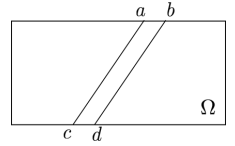
\includegraphics[width=4cm]{1.png}
	\end{minipage}
\end{figure}

\noindent (a) (1 point) Consider the diffusion equation
$$
\nabla \cdot(d \nabla u)=0, \quad x \in \Omega
$$
Impose Dirichlet boundary conditions
$$
\left.u\right|_{x=-1}=1,\left.\quad u\right|_{x=1}=0
$$
on the left and right boundaries, respectively, and Neumann- 0 boundary conditions
$$
\left.u_{y}\right|_{y=-0.5}=0,\left.\quad u_{y}\right|_{y=0.5}=0
$$
on the other parts of the boundary. Explain, how these conditions can be interpreted physically. What impact do they have if applied to a biological diffusion problem like the drug penetration into the skin?\\

\noindent Solution:\\
\noindent Dirichlet boundary conditions mean the diffusion density on the left equals to 1 and that on the right equals to 0. Neumann boundary conditions mean the gradient of diffusion density along y direction on the upper and lower boundary equal to 0. The greater the drug density the larger the value of Dirichlet boundary condition on the left boundary. \\

\noindent (c) (2 points) Perform simulations of the diffusion described by this problem using the script $diffusion\_with\_stripe.lua$. Set the diffusion coefficient $d=1$ in $\Omega \backslash a b d c$. Try to different values $d=0.0001$ and $d=0.1$ in the stripe $a b d c$ (used the option -stripeD). Visualize your results with ParaView. Compare your two solutions and explain your observations physically by adressing both, the different diffusion coefficients and the boundary conditions.\\

\noindent Solution:\\
\noindent The results are shown in Fig.1 and 2. A low diffusion coefficient stripe will block the drug from left to right. A high diffusion coefficient stripe will allow more drug transform from left to right.\\
\begin{figure}[htbp]
	\centering
	\begin{minipage}[t]{0.7\textwidth}
		\centering		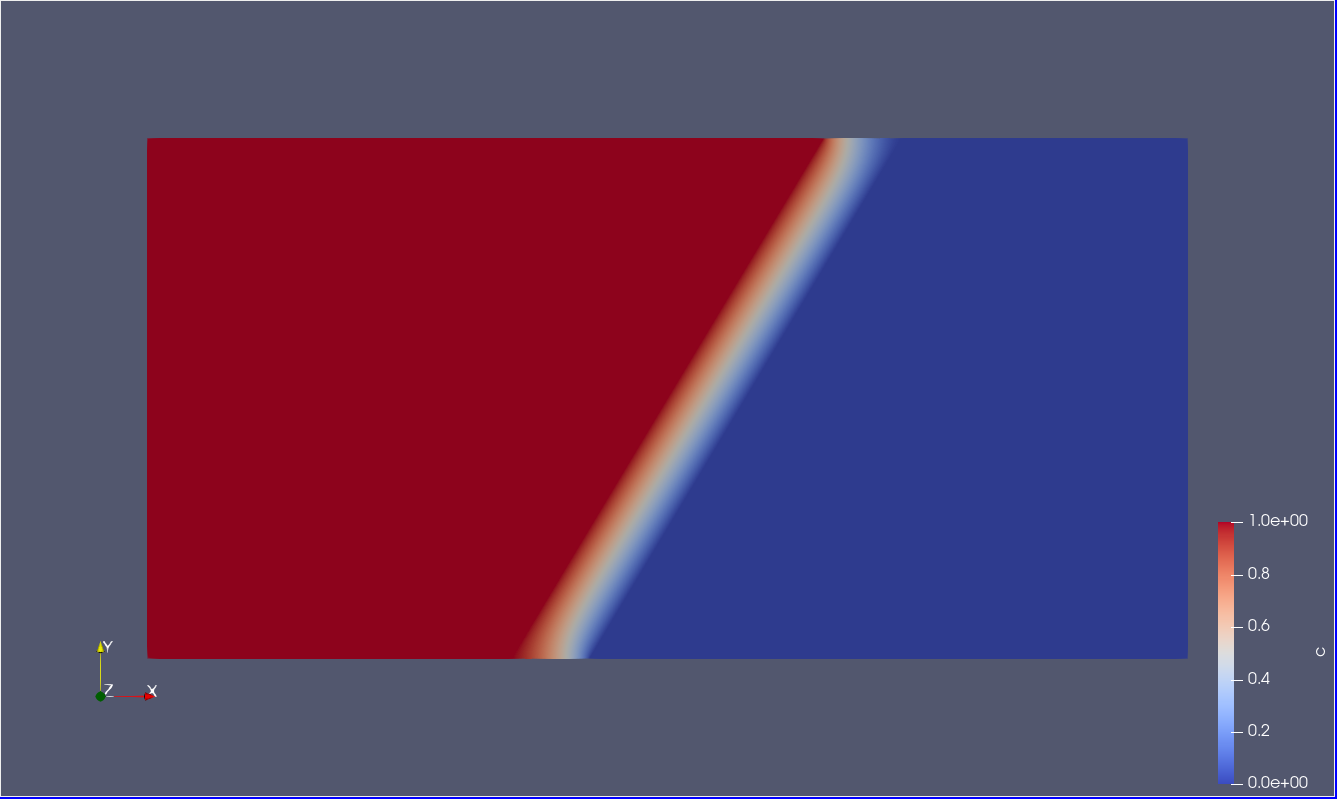
\includegraphics[width=10cm]{2.png}
		\caption{Stripe diffusion = 0.0001}
	\end{minipage}
\end{figure}
\begin{figure}[htbp]
	\centering
	\begin{minipage}[t]{0.7\textwidth}
		\centering		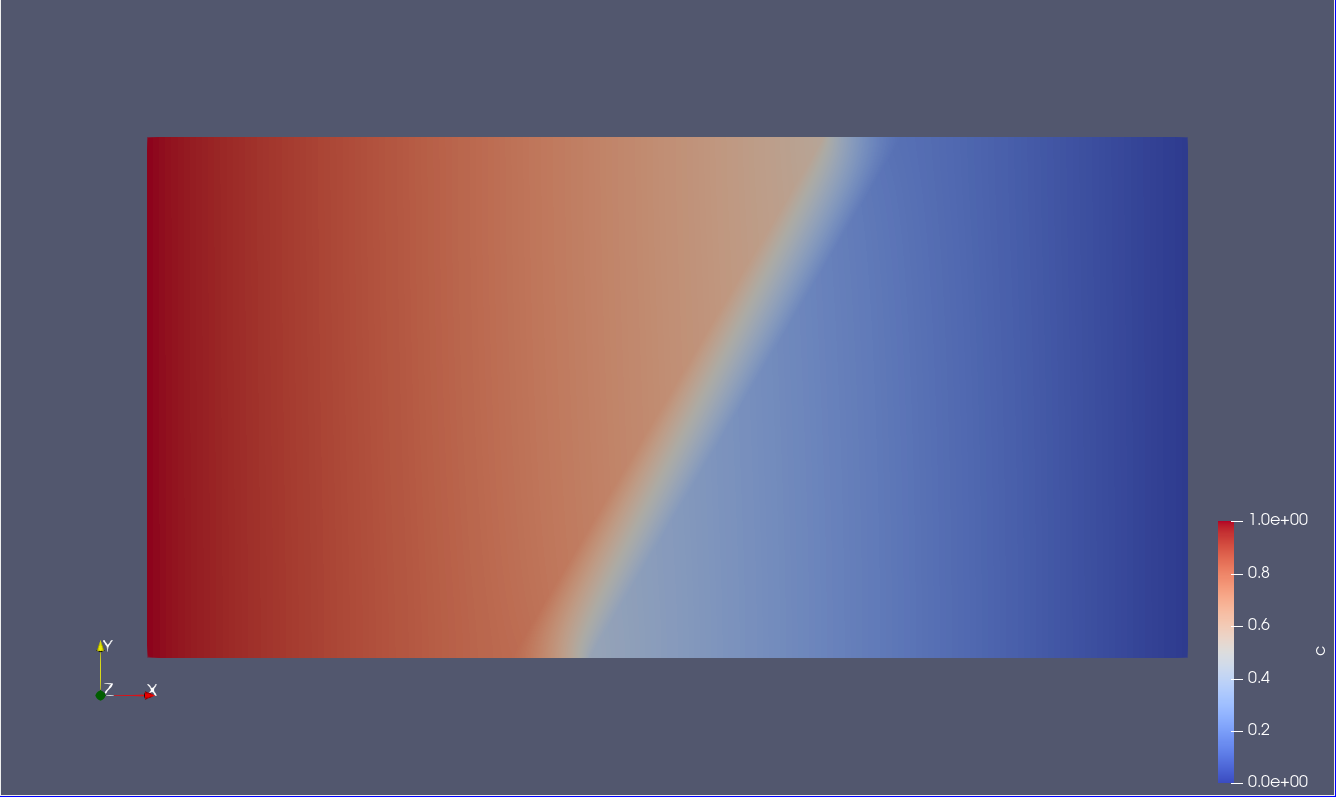
\includegraphics[width=10cm]{3.png}
		\caption{Stripe diffusion = 0.1}
	\end{minipage}
\end{figure}

\noindent \textbf{Exercise 4.2*} (a) (2 points) Perform the simulation from Exercise. 4.1(c) with $d=0.0001$ in the stripe. Compute the solution on 3 different refinement levels $(3,4$ and 5$)$ of the mesh (use the option -numRefs). As linear solver for the discrete system apply the linear iteration preconditioned by the geometric multigrid method (gmg) with the ILU smoother. For every refinement level, report the number of the degrees of freedom, the average and the last convergence rate of the iterative method, as well as number of iterations needed.\\

\noindent Solution:\\
\noindent The results are shown in Fig.3.\\
\begin{figure}[htbp]
	\centering
	\begin{minipage}[t]{0.7\textwidth}
		\centering		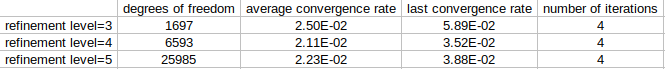
\includegraphics[width=10cm]{4.png}
		\caption{The solution on refinement level = 3, 4, 5 (gmg)}
	\end{minipage}
\end{figure}

\noindent (b) (4 points) Perform the same numerical experiments but use the linear iteration preconditioned by the ILU method. For every refinement level $i$, report the number of the degrees of freedom, the average and the last convergence rates $\left(\rho_{h, \text { ave }, i}\right.$ and $\left.\rho_{h, i}\right)$ of the iterative method, as well as number of iterations needed. Compare your results with the ones for the gmg. Explain your observations with the properties you learned about the gmg. Estimate the order of the asymptotic convergence rate w.r.t. the mesh size $h$ by comparing $\eta_{h, i}=1-\rho_{h, i}$ for different refinement levels. What does this mean for the amount of the computational work (cf. Exercise 1.4).\\

\noindent Solution:\\
\noindent The results are shown in Fig.4. The convergence rates become worse with the increase of refinement levels when using ILU method. The convergence rates is independent of refinement levels and keep on a small value when using gmg method. The comparison of $\eta_{h, i}$ is shown in Fig.5. The order of asymptotic convergence rate w.r.t. the mesh size $h$ are 0 and 2 for gmg method and ILU method respectively. The amount of the computational work of gmg method and ILU method are $O\left(h^{-2}\right)$ and $O\left(h^{-4}\right)$ respectively.\\
\begin{figure}[htbp]
	\centering
	\begin{minipage}[t]{0.7\textwidth}
		\centering		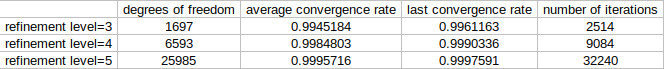
\includegraphics[width=10cm]{5.png}
		\caption{The solution on refinement level = 3, 4, 5 (ILU)}
	\end{minipage}
\end{figure}

\begin{figure}[htbp]
	\centering
	\begin{minipage}[t]{0.7\textwidth}
		\centering		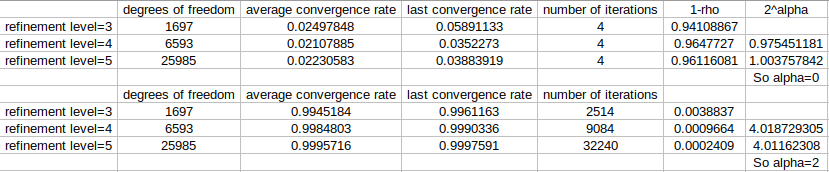
\includegraphics[width=10cm]{6.png}
		\caption{The comparison of convergence rates(Linear iteration)}
	\end{minipage}
\end{figure}

\noindent \textbf{Exercise 4.3*} ( 3 points) Perform the same experiments as in Ex. $4.2(\mathrm{a}, \mathrm{b})$ but with the cg method instead of the linear iteration. Report the average convergence rate $\rho_{h, \text { ave }, i}$ of the iterative method, as well as number of iterations needed. For the case of the plain ILU preconditioner, compute $\eta_{h, \text { ave }, i}=1-\rho_{h, \text { ave }, i}$ for the refinement levels and estimate the order of the averaged convergence rate w.r.t. the mesh size $h$.\\

\noindent Solution:\\
\noindent The results are shown in Fig.6. For the case of the plain ILU preconditioner, the order of the averaged convergence rate w.r.t. the mesh size $h$ is 1.\\
\begin{figure}[htbp]
	\centering
	\begin{minipage}[t]{0.7\textwidth}
		\centering		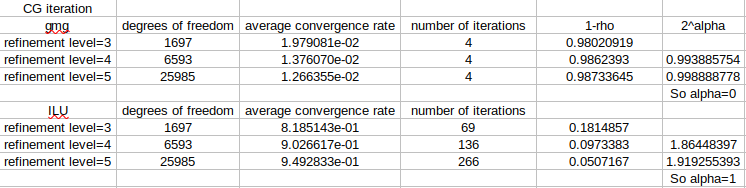
\includegraphics[width=10cm]{7.png}
		\caption{The comparison of convergence rates(CG iteration)}
	\end{minipage}
\end{figure}

\noindent \textbf{Exercise 4.4*} (4 points) Consider the boundary value problem given on the unit square by
$$
\Delta u(x, y)=f(x, y)=400[\sin (20 x)+\sin (20 y)], \quad(x, y) \in \Omega=(0,1) \times(0,1)
$$
$$
\left.u(x, y)\right|_{\delta \Omega}=\sin (20 x)+\sin (20 y)
$$
For the finite volume method, it can be proven that in the Euclidean norm, the numerical solution $u_{h}$ converges to the analytical solution $u$ with the convergence order $q=2$, i.e.
$$
\left\|u-u_{h}\right\|_{2}=O\left(h^{2}\right)
$$
Use the script $poisson\_error.lua$ to measure the order $q$ numerically: Compute the solution $u_{h_{i}}$ for 6 successive mesh refinement levels, $i=4, \ldots, 9$, with mesh sizes $h_{i}=1 / 2^{i+1}$. (Use option -numRefs.) The numerical order is given by
$$
q_{\mathrm{num}, i}:=\log \frac{\left\|u-u_{h_{i}}\right\|_{2}}{\left\|u-u_{h_{i+1}}\right\|_{2}} / \log \frac{h_{i}}{h_{i+1}}
$$
Report the error $\left\|u-u_{h_{i}}\right\|_{2}$ for each level $i$ of refinement as well as the measured numerical order of the convergence.\\

\noindent Solution:\\
\noindent The results are shown in Fig.7.\\
\begin{figure}[htbp]
	\centering
	\begin{minipage}[t]{0.7\textwidth}
		\centering		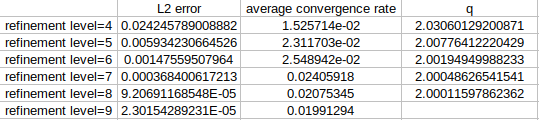
\includegraphics[width=10cm]{8.png}
		\caption{The L2 error and the numerical order of the convergence}
	\end{minipage}
\end{figure}

\end{document}.